\section{Nebulas Rank}
对应与经济模型

我们给出广泛意义上的Nebulas Rank的算法所需要满足的性质。
假设,Nebulas Rank计算函数为\(f(x)\),其中\(x\)
为Nebulas Rank需要参考的因素,可以为持有的余额、币龄或账户的出入度。为了操纵Nebulas Rank的计算,
攻击者可以进行任意的操作,包括创建足够多的账户、进行账户之间的转账等,在诸多攻击方式中,唯一确定的事实是,
{\color{red} 用户需要将原本属于一个账户的资金拆分为多份,并转移到其他账户中},因此为了抵抗操纵,
需要保证用户在拆分资金后,其Nebulas Rank会降低,即:

\begin{align}
f(a + b) > f(a) + f(b), a>0, b>0.
\end{align}

需要注意的是,上式可能会产生另外一种可能的操纵Nebulas Rank的方式,即多个用户通过将账户中的余额集中
到同一个账户中,以获得更高的收益,因此,需要满足

\begin{align}
\lim\limits_{a \to \infty, b\to \infty} f(a+b) = f(a) + f(b), a>0, b>0
\end{align}

Nebulas Rank的计算需要满足上述两个性质,我们给出一个满足上述性质的函数
\begin{align}
f(x) = x/(1 + a*e^{b + c*x})
\end{align}
\noindent 该函数的图形如\reffig{fig-nr}所示。
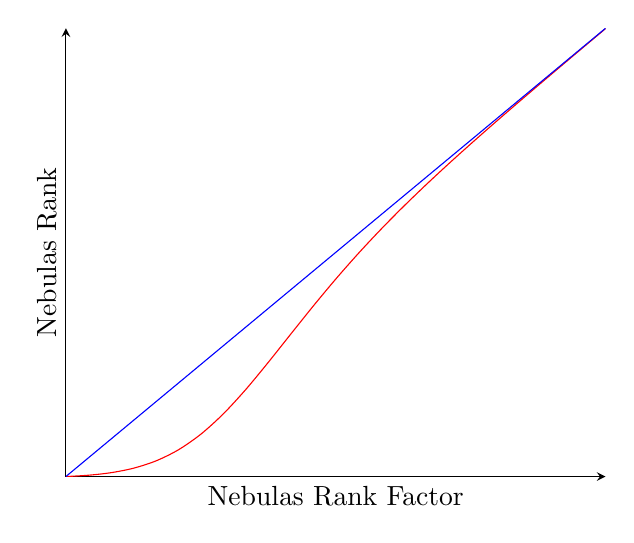
\begin{tikzpicture}[
    declare function={func(\x,\mu) = (\x / (1 + exp(\mu-\x)));},
    declare function={linefunc(\x) = \x;}
]
\begin{axis}[
    axis lines=left,
    enlargelimits=upper,
ticks=none,axis x line=bottom,axis y line=left,xlabel={Nebulas Rank Factor},
  ylabel={Nebulas Rank}
]
\addplot [smooth, domain=0:10, red] {func(x,3)};
\addplot [smooth, domain=0:10, blue] {linefunc(x)};
\end{axis}
\label{fig-nr}
\end{tikzpicture}


NR试图衡量经济流通性

然而这很困难,大牛表示,只是从图来做这个事情,是搞不定的

更进一步的,各种复杂的场景,需要的Rank非常多样化

因此,我们为白皮书中的东西,定义为NR Core,更广义的使用场景,定义为NR Extension
